
\documentclass{llncs}
%\usepackage{times}
\usepackage{epsfig}
%\usepackage{enumerate}
%\usepackage{paralist}
%\usepackage{amsmath}
%\usepackage{amssymb}
%\usepackage{amscd}
%\usepackage{array}
%\usepackage{tabularx}
\usepackage{xspace}
\usepackage{url}
%\usepackage{float}
\usepackage{multirow}
\usepackage{listings}
%\usepackage{latexsym,pstricks,pst-node,pst-tree,boxedminipage,stmaryrd}
%\usepackage{alltt}
%\usepackage{fancyhdr}
%\usepackage{fullpage}

\usepackage{paralist}
%\markboth{INSPIRED}{INSPIRED}

%\pagestyle{myheadings}

% julien: mes macros
\newcommand{\rarrow}{$\rightarrow$}
\newcommand{\conj}{$\wedge$}
\newcommand{\disjonc}{$\vee$}
\newcommand{\s}{\,}
\newcommand{\btab}{\begin{tt}\begin{tabbing}}
\newcommand{\etab}{\end{tabbing}\end{tt}}
% julien: fin de mes macros
\newcommand{\native}{\texttt{native}\xspace}

\pagestyle{plain}
\title{JACK~---~a tool for validation of security and behaviour of Java
applications\thanks{This work is partially funded by the IST programme
of the European Commission, under the IST-2003-507894
\textsf{Inspired} and IST-2005-015905 \textsf{Mobius} projects.}}

\author{Gilles Barthe\inst{1} \and
        Lilian Burdy\and %\inst{2} \and
        Julien Charles\inst{1} \and
        Benjamin Gr\'egoire\inst{1} \and
        Marieke Huisman\inst{1} \and
        Jean-Louis Lanet\inst{2} \and
        Mariela Pavlova\inst{3}\thanks{Research done while at INRIA Sophia Antipolis.} \and
        Antoine Requet\inst{2}}
\institute{INRIA Sophia Antipolis, France \and 
           gemalto, France \and 
           Ludwig-Maximilians-Universit\"at M\"unchen, Germany}


\parindent 1cm
\parskip 0.2cm
\topmargin 0.2cm
\oddsidemargin 1cm
\evensidemargin 0.5cm
\textwidth 15cm
\textheight 21cm

\def\lstlanguagefiles{lstlangjml.sty}
\lstloadlanguages{Jml}

\newcommand{\benchname}[1]{\texttt{#1}}

\newcommand{\comment}[1]{{\sf #1}}
\newcommand{\alarm}[1]{\marginpar{#1}}

\newtheorem{definition}{Definition}
\newtheorem{lemma}{Lemma}
\newtheorem{theorem}{Theorem}


\def \bsl       {\symbol{92}}
\def \unsc      {\symbol{95}}

\newcommand{\todo}[1]{ \textbf{#1}}
\newcommand{\fig}[1]{ Fig.}
\newcommand{\jmlKey}[1]{\texttt{#1}}% wrapping jml keywords
\newcommand{\java}[1]{\texttt{#1}}
\newcommand{\stack}[1]{\texttt{st(#1)}}% element on top stack 
\newcommand{\counter}{\texttt{ct}}

\newcommand{\true}{\texttt{true}}
\newcommand{\false}{\texttt{false}}

\newcommand{\wpi}{\textit{wp}}

\newcommand{\instr}[1]{\texttt{#1}}

\newcommand{\substitution}[2]{[\tt{#1} \leftarrow \tt{#2}]}
% thegrammar for the bytecode specification language
\newcommand{\ClassSpec}{\rm{ClassSpec}}
\newcommand{\MethodSpec}{\rm{MethodSpec}}
\newcommand{\SpecCase}{\textrm{SpecCase}}
\newcommand{\jmlStmt}[1]{\textrm{#1}}
\newcommand{\interMethodSpec}{\rm{InterMethodSpec}}
\newcommand{\loopSpec}{\rm{loopSpec}}
%\newcommand{\assert}{\rm{assertSpec}}

\newcommand{\ArithExpr}{\texttt{Arithmetic\_Expr}}
\newcommand{\expression}{\mathcal{E} }

\newcommand{\integer}{\texttt{int} }
\newcommand{\register}[1]{\texttt{lv[#1]} }
\newcommand{\reference}{\texttt{ref} }
\newcommand{\intLiteral}{\texttt{int\_literal} }
\newcommand{\Mynull}{\texttt{null}}
\newcommand{\this}{\texttt{this}}
\newcommand{\fieldAccess}[1]{\texttt{field\_cp\_index(}#1 \texttt{)}}
\newcommand{\arrayAccess}[2]{#1[#2] }

\newcommand{\result}{\jmlKey{$\backslash$result}}
\newcommand{\oldp}[1]{\jmlKey{$\backslash$old(}#1\jmlKey{)}}
\newcommand{\typeof}[1]{\jmlKey{$\backslash$typeof(}#1 \jmlKey{)}}
\newcommand{\EXC}{\texttt{EXC}}

\newcommand{\excPost}{\psi^{exc}}

\newcommand{\Myspace}{\phantom{aa}}
\newcommand{\predicate}{ \mathcal{P}} 
\newcommand{\Myfalse}{\textit{false}}
\newcommand{\Mytrue}{ \textit{true} }
\newtheorem{defn}{Definition} 



% abstractCtrlFlow.tex
\newcommand{\execRel}{\rightarrow} % the execution relation
\newcommand{\blockm}[1]{ \tt{b^{#1}} }
\newcommand{\blockSeq}[1]{ \tt{b_{seq}^{#1}} }
%\newcommand{\pathm}[2]{\blockm{#1} \execRel^{*} \blockm{#2} }

\newcommand{\blockPost}[1]{ \it{post(}\tt{b_{seq}^{#1}}\it{)}}

\newcommand{\invariant}{\textit{I}}

\newcommand{\srcVar}[1]{\texttt{#1} }

\newcommand{\method}{\texttt{m} }

% recuperé dans le prelude du code généré par l'Atelier B.
% Doit permettre d'écrire à peu-près correctement <+
\def\famletter#1{\ifcase #1 0\or 1\or 2\or 3\or 4\or 5\or 6\or 7\or
    8\or 9\or A\or B\or C\or D\or E\or F\fi}
\font\msx=msam10
\newfam\msxfam \textfont\msxfam=\msx
\edef\fx{\famletter\msxfam}
\mathchardef    \dres       "2\fx43
\def    \lover      {\mathbin{{\dres} \llap{$-\!\!\!\!-\!$}}}

\def\keywords{\noindent\bf Keywords: \vspace{0pt}
\it\normalsize\normalsize}
\def\endkeywords{\par}

\def\acknowledgement{\vspace{4pt} \noindent{\bf Acknowledgements} \\ \vspace{1pt}
\normalsize\normalsize}
\def\endkeywords{\par}

\newcommand{\JACK}{\texttt{JACK}}
\newcommand{\ESC}{\texttt{ESC/Java}}
\newcommand{\LOOP}{\texttt{LOOP}}


\title{Methodology for Java Application Validation}

\author{INRIA Sophia Antipolis\\Everest team}

\date{}
\newcommand{\bbb}{\mathbb{B}}
% moved here from carmel.tex
\newcommand{\spp}{\hspace{1.5cm}}


\newcommand{\semb}{\llbracket}
\newcommand{\seme}{\rrbracket}
\newcommand{\sem}[1]{ \semb #1 \seme}
\newcommand{\ia}[1]{ \semb #1 \seme}
\newcommand{\fia}[1]{ \mathcal{F}\semb #1 \seme}
\newcommand{\ria}[1]{ \mathcal{R}\semb #1 \seme}

\newcommand{\Coq}{{\sf Coq}}
\newcommand{\ocaml}{\textsc{ocaml}}

\newcommand{\memvar}{\text{Mem}}

\newcommand{\AbVal}{\widehat{\text{Val}}}
\newcommand{\Val}{{\text{Val}}}
%\newcommand{\Stack}{{\text{Stack}}}
\newcommand{\AbStack}{{\widehat{\text{Stack}}}}
\newcommand{\SafeCallStack}{{\text{SafeCallStack}}}
\newcommand{\OneCall}{{\text{OneCall}}}
\newcommand{\Var}{{\text{Var}}}
\newcommand{\LocalVar}{{\text{LocalVar}}}
\newcommand{\AbLocalVar}{{\widehat{\text{LocalVar}}}}
\newcommand{\State}{{\text{State}}}
\newcommand{\Trace}{{\text{Trace}}}
\newcommand{\AbState}{{\widehat{\text{State}}}}
\newcommand{\progCount}{{\text{progCount}}}
\newcommand{\fieldName}{{\text{fieldName}}}
\newcommand{\methodName}{{\mathrm{methodName}}}
\newcommand{\MM}{{\methodName}}
\newcommand{\PP}{{\progCount}}
\newcommand{\className}{{\text{className}}}
\newcommand{\varName}{{\text{varName}}}
\newcommand{\Adress}{{\text{Adress}}}
\newcommand{\Instruction}{{\text{Instruction}}}
\newcommand{\InstAt}{{\text{InstAt}}}
\newcommand{\Constraint}{{\text{Constraint}}}
\newcommand{\St}{\widehat{\text{St}}}

\newcommand{\config}[1]{{\langle\!\langle #1 \rangle\!\rangle}}
\newcommand{\fram}[1]{{\left\langle #1 \right\rangle}}
\newcommand{\num}{{\text{num}}}
\newcommand{\reff}{{\text{ref}}}
\newcommand{\nul}{{\text{null}}}
\newcommand{\some}{{\text{some}}}
\newcommand{\nameClass}{{\text{nameClass}}}
\newcommand{\class}{{\text{class}}}
\newcommand{\newObject}{{\text{newObject}}}
\newcommand{\newArray}{{\text{newArray}}}
\newcommand{\lengthArray}{{\text{lengthArray}}}
\newcommand{\fieldValue}{{\text{fieldValue}}}
\newcommand{\Value}{{\text{Value}}}
\newcommand{\classes}{{\text{classes}}}
\newcommand{\RefValue}{{\text{RefValue}}}
\newcommand{\Location}{{\text{Location}}}
\newcommand{\methodLookup}{{\text{methodLookup}}}
\newcommand{\nbArgument}{{\text{nbArgument}}}
\newcommand{\nameMethod}{{\text{nameMethod}}}

\newcommand{\ClassName}{{{\text{ClassName}}}}
\newcommand{\FieldName}{{{\text{FieldName}}}}
\newcommand{\default}{{{\text{default}}}}
\newcommand{\END}{{{\text{END}}}}
\newcommand{\AbHeap}{{\widehat{\text{Heap}}}}

\newcommand{\Sinit}{{\mathcal{S}_{\mathit{init}}}}

\newcommand{\instructionAt}{{\text{instructionAt}}}


%\newcommand{\abs}{\mbox{${\cal S}\!\mathit{t}$}}
\newcommand{\abs}{\mbox{$\Sigma$}}
\newcommand{\addr}{\mbox{\em addr}}
\newcommand{\pc}{\mathit{pc}}
\newcommand{\stf}{{\mathit{sf}}}
\newcommand{\cl}{{\mathit{cl}}}

\newcommand{\analyze}{\text{\tt analyse}}
\newcommand{\Analyze}{\ensuremath{\mathit{Unbounded}(P)}}
\newcommand{\Program}{\text{Program}}

\newenvironment{constraint}{%
\noindent
\hspace{.3mm}$
\begin{array}[t]{l}}{%
\end{array}$\\[0.2cm]
}

\newenvironment{contraint}{%
\noindent
\hspace{1cm}$
\begin{array}[t]{l}}{%
\end{array}$\\[0.5cm]
}




\newcommand{\AbPop}{\widehat{\text{pop}}}
\newcommand{\AbPush}{\widehat{\text{push}}}
\newcommand{\AbTop}{\widehat{\text{top}}}
\newcommand{\AbBinop}{\widehat{\text{binop}}}
\newcommand{\AbApply}{\widehat{\text{apply}}}
\newcommand{\AbSubst}{\widehat{\text{subst}}}
\newcommand{\Num}{{{\text{Num}}}}
\newcommand{\AbNum}{{\widehat{\text{Num}}}}
\newcommand{\AbRef}{{\widehat{\text{Ref}}}}
\newcommand{\AbObject}{{\widehat{\text{Object}}}}
%\newcommand{\AbHeap}{{\widehat{\text{Heap}}}}
\newcommand{\Flow}{\text{\tt Flow}}

\newenvironment{myalltt}{\vspace*{-3pt}\begin{alltt}}{\end{alltt}\vspace*{-3pt}}

%%
%% Added by Gerardo (28/09/2004)
%%

\newcommand{\Rule}[2]
{
\frac{#1}
{
\begin{array}{l}
#2
\end{array}
}
}

\newcommand\Loop{\ensuremath{\mathit{Loop}}}
\newcommand\Pred{\ensuremath{\mathit{Pred}}}
\newcommand\BC{\ensuremath{\mathit{BC}}}
\newcommand\MutRec{\ensuremath{\mathit{MutRecR}}}
\newcommand\Rec{\ensuremath{\mathit{Rec}}}
\newcommand\Anc{\ensuremath{\mathit{Anc}}}
\newcommand\LoopCall{\ensuremath{\mathit{LoopCall}}}
\newcommand\Call{\ensuremath{\mathit{Call}}}
\newcommand\Q{\ensuremath{\mathit{Q}}}
\newcommand\tr{\ensuremath{\mathit{tr}}}

\newcommand\End{\ensuremath{\mathtt{end}}}
\newcommand\nop{\ensuremath{\mathtt{nop}}}
\newcommand\push{\ensuremath{\mathtt{push}}}
\newcommand\pop{\ensuremath{\mathtt{pop}}}
\newcommand\dup{\ensuremath{\mathtt{dup}}}
\newcommand\swap{\ensuremath{\mathtt{swap}}}
\newcommand\numop{\ensuremath{\mathtt{numop}}}
\newcommand\load{\ensuremath{\mathtt{load}}}
\newcommand\store{\ensuremath{\mathtt{store}}}
\newcommand\inc{\ensuremath{\mathtt{inc}}}
\newcommand\add{\ensuremath{\mathtt{add}}}
\newcommand\sub{\ensuremath{\mathtt{sub}}}
\newcommand\goto{\ensuremath{\mathtt{goto}}}
\newcommand\If{\ensuremath{\mathtt{if}}}
\newcommand\looksw{\ensuremath{\mathtt{lookupswitch}}}
\newcommand\tabsw{\ensuremath{\mathtt{tableswitch}}}
\newcommand\newarray{\ensuremath{\mathtt{newarray}}}
%\newcommand\default{\ensuremath{\mathtt{default}}}
\newcommand\new{\ensuremath{\mathtt{new}}}
\newcommand\checkc{\ensuremath{\mathtt{checkcast}}}
\newcommand\getst{\ensuremath{\mathtt{getstatic}}}
\newcommand\putst{\ensuremath{\mathtt{putstatic}}}
\newcommand\instof{\ensuremath{\mathtt{instanceof}}}
\newcommand\getfd{\ensuremath{\mathtt{getfield}}}
\newcommand\getfdt{\ensuremath{\mathtt{getfield this}}}
\newcommand\putfd{\ensuremath{\mathtt{putfield}}}
\newcommand\invdef{\ensuremath{\mathtt{invokedefinite}}}
\newcommand\invvir{\ensuremath{\mathtt{invokevirtual}}}
\newcommand\invint{\ensuremath{\mathtt{invokeinterface}}}
\newcommand\return{\ensuremath{\mathtt{return}}}
\newcommand\arrlh{\ensuremath{\mathtt{arraylength}}}
\newcommand\arrld{\ensuremath{\mathtt{arrayload}}}
\newcommand\arrst{\ensuremath{\mathtt{arraystore}}}
\newcommand\throw{\ensuremath{\mathtt{throw}}}
\newcommand\jsr{\ensuremath{\mathtt{jsr}}}
\newcommand\ret{\ensuremath{\mathtt{ret}}}
\newcommand\thiss{\ensuremath{\mathtt{this}}}
%\newcommand\instr{\ensuremath{\mathtt{instr}}}
\newcommand\const{\ensuremath{\mathtt{const}}}
\newcommand\Array{\ensuremath{\mathsf{array}}}
\newcommand\Int{\ensuremath{\mathsf{int}}}
\newcommand\byte{\ensuremath{\mathsf{byte}}}
\newcommand\short{\ensuremath{\mathsf{short}}}
\newcommand\bool{\ensuremath{\mathsf{bool}}}
\newcommand\Ctxt{\ensuremath{\mathsf{Ctxt}}}

\newcommand\warn{\ensuremath{<!>}}
\newcommand\trace{\overline{s}}
\newcommand\defi{\stackrel{\mathrm{def}}{=}}
\newcommand\lub{\sqcup}

\newcommand\Size{\ensuremath{\mathit{Size}}}
\newcommand\Pre{\ensuremath{\mathrm{Pre}}}
\newcommand\Post{\ensuremath{\mathrm{Post}}}
\newcommand\old{\ensuremath{\backslash\mathrm{old}}}

%%%%%%%%%%%%%%%%%%%%%%%%%%%%%%%%%%%%%%%%%%%%%%%%%%%%%%%
%%
%% Mariela's definitions
%%
%%%%%%%%%%%%%%%%%%%%%%%%%%%%%%%%%%%%%%%%%%%%%%%%%%%%%%%


%\newcommand{\pathm}[2]{\blockm{#1} $\ll^{*}$ \blockm{#2} }



%%%%%%%%%Specification commands
\newcommand{\annotation}{BML}
\newcommand{\Apredicate}{\textit{P}}


\newcommand{\requires}{\texttt{requires}}
\newcommand{\ensures}{\texttt{ensures}}
\newcommand{\exsures}[1]{\texttt{exsures(#1)}}
\newcommand{\assert}{\texttt{assert}}

\newcommand{\variant}{\texttt{variant}}

\newcommand{\declare}{\texttt{declare}}
\newcommand{\ghost}{\texttt{Model}}
\newcommand{\ghostSet}{\texttt{set}}
\newcommand{\modifies}{\texttt{modifies}}
\newcommand{\ensemble}[2]{#1 .. #2}
\newcommand{\maxIter}[1]{ iter^#1 }
\newcommand{\progLoop}[1]{\textit{#1}}
\newcommand{\memConsAt}[1]{\Mem^l}

\newcommand{\atState}[2]{#1^{#2} }

%\newcommand{\Mem}{\texttt{MemUsed}}
\newcommand{\Mem}{\texttt{Mem}}
%\newcommand{\old}{\texttt{old}}
\newcommand\Max{\ensuremath{\texttt{Max}}}
\newcommand{\allocated}[1]{allocPath(#1)}
\newcommand{\srcCode}[1]{\texttt{#1}}
\newcommand{\local}[1]{\texttt{localVar}(#1)}



%%%%%%%%%%%% allocation function
\newcommand{\visited}{\texttt{visited}}



%\newcommand{\instrAt}[1]{i_{#1}}
%\newcommand{\instanceOfAlloc}[1]{instanceOfAllocates( #1 )}

\newcommand{\allocInstance}[1]{\texttt{allocInst(#1)}}
\newcommand{\allocLoop}[1]{\texttt{loopCon(#1)}} % function that returns directly the allocations done by a loop : multiplied by the max iterations it can do
\newcommand{\allocMethod}[1]{\texttt{mthdCon(#1)}} % returns the allocations done in a method
\newcommand{\allocLoopWithEnd}[2]{alloc\_loop\_path(#1 , #2)} % returns the allocations done in a loop for a particular path that starts at the start instruction of a loop and that % ends with an insstruction that leads back to the start instructions

\newcommand{\allocIns}[1]{alloc\_instr(#1)} % function that returns that the allocation by the argument

\newcommand{\numLoop}[1]{\textit{numberLoop}(#1)}
\newcommand{\loopEndsSet}[1]{loopEndSet(#1)}
\newcommand{\loopSet}[1]{loopSet(#1)}
\newcommand{\loopEntry}[1]{entry(#1)} % predicate that says that the instruction is an entry to a loop

\newcommand{\backedge}[2]{backedge(#1,#2)} % the start of the backedge  and the end of the backedge


%\newcommand{\wpi}[3]{ \rm{wp}( \srcCode{#1}, #2, #3) } % wp for instructions
\newcommand{\wpExe}[1]{ \rm{wp}(#1) } % wp for blocks
\newcommand{\normalPost}{\psi^{n}}


%\newcommand{\stack}[1]{St(#1)}
\newcommand{\topStack}{c}
\newcommand{\javaNull}{null}
\newcommand{\Ref}[1]{ref_{#1} }
\newcommand{\NULL}{\texttt{null}}



\newcommand{\prevIns}[1]{prev(#1 )}
\newcommand{\nextIns}[1]{next(#1 )}
\newcommand{\targetIns}[1]{target(#1)}



%%%%%%%%%%%%%%%%%%%%%%%%%%%%%%%%%%%%%%%%%%%%%%%%%%%%%


          % input user-defined commands

\begin{document}
\maketitle      
\begin{abstract}
We describe the main features of JACK (Java Applet Correctness Kit), a
tool for the validation of Java applications, annotated with JML
specifications. JACK has been especially designed to improve the
quality of trusted personal device applications. JACK is fully
integrated with the IDE Eclipse, and provides an easily accessible
user interface. In particular, it allows to inspect the generated
proof obligations in a Java syntax, and to trace them back to the
source code that gave rise to them. Further, JACK provides support for
annotation generation, and for interactive verification. The whole
platform works both for source code and for bytecode, which makes it
particularly suitable for a proof carrying code scenario.
\end{abstract}
\section{Introduction}


Smart cards are trusted personal devices whose characteristics are
regulated by the ISO 7816 standard. As other trusted personal devices,
smartcards are designed to store and process confidential data, and
can act as tokens to provide users with a secure electronic
representation in a large network. They are widely deployed and used
in application areas such as mobile telecommunications, banking,
transportation, electronic identity, and digital rights management
(DRM). Further, they hold the promise to play a key role in the
e-society, especially as a means to guarantee users a personalized,
global, and secure access to applications and services.


The prominent role played by trusted personal devices in security
sensitive applications make them an ideal target for
attacks. Traditionally, the main concern with smartcards has been with
hardware attacks in which the attacker gains access to confidential
information or disturbs the functioning of the card through
observation (e.g. of power or electro-magnetic radiations) or invasion
(e.g. overriding sensors or attaching probes). This issue is studied in
Deliverable D8.1.

The trusted personal device remains a specific domain where post
issuance corrections are very expensive due to the deployment process
and the mass production. Furthermore, the emergence of new generation
trusted personal devices increasingly connected to networks and
providing execution support for complex programs and the prospect of
logical attacks has urged the trusted personal devices industry to
improve the quality of their software, as logical attacks are
potentially easier to launch than physical attacks (for example they
do not require physical access to the device, and are easier to
replicate from one device to the other), and may have a huge impact.
In particular, a malicious attacker spreading over the network and
disconnecting or disrupting devices massively could have deep consequences.

This deliverable reports on the development of methodologies and tools
that increase confidence in applications.  For concreteness, we focus 
on Java applications that can be executed on devices that embed Java
Virtual Machines (JVM) or their variants, in particular Java Card
Virtual Machines (JCVM). Java enabled devices are a natural choice for
formal methods because:
\begin{inparaenum}[i)]
\item they are widely deployed in the field;
\item they feature mechanisms that contribute to the security of the
platform and the applications that execute over it;
\item detailed informal specifications of the Java platform are publicly
available, and can be scrutinized.
\end{inparaenum}
However, it should be clear that the methods presented in this document
are relevant to other execution platforms for trusted personal devices.


\subsection{Security issues}
While the focus of the deliverable is on application validation,
security is a holistic property of a system, and formal techniques
must therefore be employed at different levels to provide strong
guarantees about the security of a TPD and its applications.
Essentially, the levels are: the hardware, platform, the libraries,
and the applications.

The need to consider security at those levels is illustrated for
example by the case study described on Page 55 in Deliverable D8.2,
which is concerned with secure platforms. The development of secure
API is discussed in Deliverables D7.1 and D7.2. As previously mentioned,
hardware security is discussed in Deliverable D8.1.


\paragraph*{Platform} The TPD security architecture guarantees that
downloaded applications are innocuous and comply with some basic
policies related to typing, initialization or access control. Such
basic policies are the cornerstones upon which the overall security of
the smartcard will rely. Therefore it is important to verify that the
security architecture does enforce these basic policies as
intended. Thus, an important application of formal methods to TPD
security is platform verification, which aims at providing an abstract
model of the Java platform and security architecture, and at proving
that the security functions play their expected role.

\paragraph*{Libraries} However, it is not sufficient to show that
security functions are correctly designed. In particular, one also has
to ensure that other components of the infrastructure, in particular
API, are correctly designed and implemented. For the purpose of this
deliverable, where the focus is on Java based TPD, the Java API and
the Global Platform API constitute two prominent components of the
infrastructure whose correct design is central to security. 


\paragraph*{Applications} 
Platform and libraries verification is a fundamental step towards
guaranteeing the security of smartcards, and a prerequisite for Common
Criteria evaluations at the highest levels. Nevertheless, the
guarantees offered by the Java security architecture are limited, and
further verifications must be performed to verify that applications
make a legitimate use of the infrastructure, and do not attempt any
hostile action.

Thus, application validation is another important application of
formal methods to TPD security. To date, testing campaigns remain the
primary means to ensure the quality of applications. However, testing
campaigns are expensive and only provide partial guarantees with
regard to the reliability of software. Therefore, it is important to
develop other advanced techniques for applet validation.

There are many facets to applet validation, each with its own
objectives and techniques:
\begin{itemize}
\item one can enhance existing security architectures to enforce
security properties not addressed by current architectures, in
particular confidentiality and availability.  Verification can be
performed by enhanced bytecode verification mechanisms;


\item one can abandon the realm of type systems and its associated
benefits and choose develop logical methods for specifying and
verifying either automatically or efficiently a specific class of
security properties. Verification can be performed by (possibly
efficient and hence incomplete) logic-based proof inference
mechanisms;




\item one can exploit the expressive power of logical methods to
require that applications, or at least sensitive fragments of
applications, are subjected to functional verification, i.e. to
verifications that establish their correctness in terms of
functionality as well as security.
\end{itemize}



\subsection{Logical verification of security properties using JML}
In order to provide precise analyzes with a limited overhead, we
advocate an integrated approach where validation techniques of
increasing strength are used, starting from automated techniques such
as testing and moving towards formal validation using a combination of
automated and interactive tools. In addition, we aim at overcoming the
difficulty of introducing formal techniques in industrial processes by
providing notations and tools hiding the mathematical formalisms and
by integrating formal techniques into classical developers environment
so as to allow users to benefit from formal techniques without having
to learn new formalisms and to become experts.

All the tools and results presented in this document were developed
with this goal in mind, notably the choice of JML as assertion
language and the development of JACK and its associated feature.
Using those techniques, Java developers should be able to validate
their code, or at least to get a good assurance on its correctness.


\subsubsection{JML}
JML~\cite{Leavens-Baker-Ruby99b,Leavens-Baker-Ruby03}, the ``Java
Modeling Language'', is a behavioral interface specification language
for Java; that is, it specifies both the behavior and the syntactic
interface of Java code.  The syntactic interface of a Java class or
interface consists of its method signatures, the names and types of
its fields, etc.  This is what is commonly meant by an application
programming interface (API).  The behavior of such an API can be
precisely documented in JML annotations; these describe the intended
way that programmers should use the API.  In terms of behavior, JML
can detail, for example, the preconditions and postconditions for
methods as well as class invariants. These specifications are given as
annotations of the Java source file. More precisely, they are included
as special Java comments, either after the symbols \lstinline!//@! or
enclosed between \lstinline!/*@! and
\lstinline[basicstyle=\normalfont\ttfamily\small\sl]!@*/!. For example,
the general schema for the annotation of a method is the following:
\begin{lstlisting}
/*@ behavior
  @   requires <precondition>;
  @   ensures <postcondition if no exception raised>;
  @   signals(E) <postcondition when exception E raised>;
  @   assignable <modified fields and variables>;
  @*/
\end{lstlisting}
where \lstinline!requires! specifies the conditions on variables, fields
and method parameters at the beginning of the method call so that the
conditions after \lstinline!ensures! hold at the end of the method
call and the conditions after \lstinline!signals(E)! hold if an
exception is raised and not caught inside the analyzed method.  The
underlying model is a an extension of Hoare-Floyd logic: if the
precondition holds at the beginning of the method call, then
postconditions (with and without exceptions) will hold after the
call. The \lstinline!assignable! clause specifies side-effect affected
variables and is used during the weakest precondition calculus for
method invocations.

An important goal for the design of JML is that it should be easily
understandable by Java programmers. This is achieved by staying as
close as possible to Java syntax and semantics.  Another important
design goal is that JML {\em not} impose any particular design method
on users; instead, JML should be able to document Java programs
designed in any manner \cite{Leavens-Baker-Ruby03}.

JML uses Java's expression syntax in assertions,
thus JML's notation is easy for programmers to learn.  
Because JML supports quantifiers such as
\verb_\forall_ and \verb_\exists_, and because JML allows ``model''
(i.e., specification-only) fields and methods, specifications can
easily be made precise and complete.
JML assertions are written as special
annotation comments in Java code,
so that they are ignored by Java compilers but can be used
by tools that support JML\@.  Within annotation comments JML extends the
Java syntax with several keywords.  It also extends Java's expression syntax with several
operators.
The central ingredients of a JML specification are preconditions
(given in {\tt requires} clauses), postconditions (given in {\tt
  ensures} clauses), and (class and interface) invariants.  These are
all expressed as boolean expressions in JML's extension to Java's
expression syntax.
In addition to ``normal'' postconditions, the language also supports
``exceptional'' postconditions, specified in {\tt signals} clauses.
These can be used to specify what must be true when a method throws an
exception. 

\paragraph*{Styles of specification}
Due to its expressiveness and versatility, the JML specification
language supports several styles of specifications; the choice of one
style of specification over the others depends on the purpose of the
verification effort. In a nutshell, one can either opt for lightweight
specifications in which one introduces enough annotations to reason
about some specific safety property, such as the absence of
exceptions, or heavyweight specifications where functional behavior is
considered. There is of course a great liberty in how \lq\lq
lightweight\rq\rq\ or \lq\lq heavyweight\rq\rq\ a specification should
be, and different styles can be used in different parts of an
application.

In addition, one may opt for defensive specifications, in which methods
are annotated with preconditions that prevent exceptions to occur, or
offensive specifications, which use appropriate clauses to specify 
exceptional postconditions.

\subsubsection{Verification techniques and tools}

JML specifications correctness can be verified either during runtime
or statically~\cite{BurdyCCEKLLP03}. To be verified during runtime, the
source code must have been compiled using \texttt{jmlc}, which is a
enhanced Java compiler for JML annotated code. This compiler adds to
the generated program assertions checking instructions corresponding
to the JML specifications of the program: preconditions, postconditions 
and loop or class invariants. An exception is raised during the execution 
if a JML condition fails. The JML runtime assertion checker can be used
for unit testing~\cite{CL02:ecoop}.


For the static verification of Java programs, several tools are
available using (variations of) JML as specification language. These
tools adopt different compromises between soundness and automation,
and thus it is useful to use them in combination, starting from
automatic but unsound tools, and pursuing with sound but interactive
tools.  Among these tools, ESC/Java2~\cite{CK04:cassis} offers the higher
level of automation as it does not require any user interaction and
relies on the Simplify automatic prover. It is particularly useful for
checking null pointers or array bounds limits; however it is unsound
and incomplete.

In order to further increase the level of reliability of applications,
we propose a methodology based on static verification using
JACK~\cite{BRL-JACK}, a tool that generates proof obligations that
can be discharged using proof assistants or automatic provers.


\subsection{Main contributions}
The work reported in this deliverable builds upon the JACK tool,
that was initially developed within Gemplus. The tool development
was transferred to INRIA at the beginning of the project, with
the objective to improve and increase its functionalities so as
to address the needs of INSPIRED. The main contributions of the
work carried within INSPIRED are:
\begin{itemize}
\item support for verifying high-level security properties
\item support for verifying bytecode programs
\item validation of the methodology for estimating resource
usage and optimizing code for low-footprint.
\end{itemize}
In order to carry the above tasks and evaluations, it has also
been necessary to make many improvements to the tool itself.
It is not in the scope of the present document to describe these 
improvements.


\subsection{Contents of the deliverable}
This document is organized as follows, the next chapter introduce the
assertion language JML, chapter 2 describes the JACK tool with its
extension feature, chapter 3 presents some evaluations done with the
tools and the last chapter concludes.
        
\chapter{Java Validation}
This chapter gives an overview of the JML language and the tools that have been developed to deal with the it.

\section{Java and JavaCard}
 Formal validation of Java programs is a growing research
 field.  As Java has become a reference language, many technologies are
 emerging to help Java program validation.  Java can also be
 considered as a good support for formal techniques, as it has precise 
semantics \cite{Gosl00a}.

JavaCard is a popular programming language for multiple
application smart cards.  According to the JavaCard Forum \footnote{http://www.javacardforum.org},
which involves key players in the field of smart cards, 
including smart card manufacturers and banks, the JavaCard language has two
important features that make it the ideal choice for smart cards: 
\begin{itemize}
\item JavaCard programs are written in a subset of Java, using
the JavaCard APIs (Application Programming Interfaces). JavaCard
developers can therefore benefit from the well-established Java technology; 

\item the JavaCard security model enables multiple applications to
coexist  on the same card and communicate securely, and in principle,
enables new applications to be loaded on the card after its issuance.
\end{itemize}
Yet recent research has unveiled several problems in the JavaCard
security model, most notably with object sharing and the associated
mechanism of shareable interfaces.
This has  emphasized the necessity to develop environments for
verifying the security of the JavaCard platform and of JavaCard
programs.  Thus far JavaCard security (and also Java security) has
been studied  mainly at two levels:    
\begin{itemize}
\item  platform level: here the goal is to prove safety properties of
the language, in particular type safety and properties related to
memory management; 
\item  application level: here the goal is to prove that a specific
program obeys a given property, and in particular that it satisfies a
security policy, for example based on information flow. 
\end{itemize}
We are focusing at the application level, developing tools and methodologies based on JML to reach this goal.
\section{JML}
JML~\cite{Leavens-Baker-Ruby99b,Leavens-Baker-Ruby03}, the
``Java Modeling Language'', is a behavioral interface
specification language for Java; that is, it specifies both the behavior
and the syntactic interface of Java code.  The syntactic interface of
a Java class or interface consists of its method signatures,
the names and types of its fields, etc.
This is what is commonly meant by an application programming
interface (API).
The behavior of such an API can be precisely documented in JML annotations;
these describe the intended way that programmers should
use the API.  In terms of behavior, JML can detail, for example, the
preconditions and postconditions for methods as well as class
invariants.

An important goal for the design of JML is that it should be easily
understandable by Java programmers. This is achieved by staying as
close as possible to Java syntax and semantics.  Another important
design goal is that JML {\em not} impose any particular design method
on users; instead, JML should be able to document Java programs
designed in any manner \cite{Leavens-Baker-Ruby03}.

JML uses Java's expression syntax in assertions,
thus JML's notation is easy for programmers to learn.  
Because JML supports quantifiers such as
\verb_\forall_ and \verb_\exists_, and because JML allows ``model''
(i.e., specification-only) fields and methods, specifications can
easily be made precise and complete.
JML assertions are written as special
annotation comments in Java code,
so that they are ignored by Java compilers but can be used
by tools that support JML\@.  Within annotation comments JML extends the
Java syntax with several keywords.  It also extends Java's expression syntax with several
operators.
The central ingredients of a JML specification are preconditions
(given in {\tt requires} clauses), postconditions (given in {\tt
  ensures} clauses), and (class and interface) invariants.  These are
all expressed as boolean expressions in JML's extension to Java's
expression syntax.
In addition to ``normal'' postconditions, the language also supports
``exceptional'' postconditions, specified in {\tt signals} clauses.
These can be used to specify what must be true when a method throws an
exception. 

%=====================================================================
%=====================================================================
\subsection{The JML tool suite}
\label{tools}

Since JML specifications are meant to be read and written by ordinary
Java programmers, it is important to support the conventional ways
that these programmers create and use documentation.  Consequently,
the {\tt jmldoc} tool
produces browsable HTML pages containing both the
API and the specifications for Java code, in the style of pages
generated by Javadoc~\cite{Friendly95}.

%=====================================================================
The JML compiler (\texttt{jmlc}), developed at Iowa State University,
is an extension to a Java compiler and compiles Java programs
annotated with JML specifications into Java
bytecode~\cite{Cheon03,Cheon-Leavens02b}.  The compiled bytecode includes
runtime assertion checking instructions that check JML specifications
such as preconditions, normal and exceptional postconditions,
invariants, and history constraints.  The execution of such assertion
checks is transparent in that, unless an assertion is violated, and
except for performance measures (time and space), the behavior of the
original program is unchanged.  The transparency of runtime assertion
checking is guaranteed, as JML assertions are not allowed to have any
side-effects~\cite{Leavens-etal03a}.




\section{ESC/Java2}
\label{escjava}

ESC/Java2 tool~\cite{Flanagan-Et-Al02}, originally developed at Compaq Research,
performs what is called ``extended static
checking''~\cite{ESC:Overview,10yearsESC},
compile-time checking that goes well beyond type checking.  It can
check relatively simple assertions and can check for certain kinds of
common errors in Java code, such as dereferencing \texttt{null},
indexing an array outside its bounds, or casting a reference to an
impermissible type.  ESC/Java2 supports a subset of JML and also checks
the consistency between the code and the given JML annotations.  The
user's interaction with ESC/Java2 is quite similar to the interaction
with the compiler's type checker: the user includes JML annotations in
the code and runs the tool, and the tool responds with a list of
possible errors in the program.

JML annotations affect ESC/Java2 in two ways.  First, the given JML
annotations help ESC/Java2 suppress spurious warning messages.   Second,
annotations make ESC/\-Java2 do additional checks.  
In these two ways, the use of JML annotations enables ESC/Java2 to
produce warnings not at the source locations where errors manifest
themselves at runtime, but at the source locations where the errors
are committed.

%=====================================================================
%\section{Applications of JML to Java Card}
%\label{applications}

%Although JML is able to specify arbitrary sequential Java programs,
%most of the serious applications of JML and JML tools up to now
%have targeted Java Card.  Java Card$^{TM}$ is a dialect of Java specifically
%designed for the programming of the latest generation of smartcards.
%Java Card is adapted to the hardware limitations of smartcards; for
%instance, it does not support floating point numbers, strings, object
%cloning, or threads.

%Java Card is a well-suited target for the application of formal
%methods.  It is a relatively simple language with a restricted API\@.
%Moreover, Java Card programs, called ``applets'', are small, typically
%on the order of several KBytes of bytecode.  Additionally, correctness
%of Java Card programs is of crucial importance, since they are used in
%sensitive applications such as bank cards and mobile phone SIMs.  (An
%interesting overview of security properties that are relevant for Java
%Card applications is available~\cite{MarletLM01}.)

%JML, and several tools for JML, have been used for Java Card,
%especially in the context of the EU-supported project VerifiCard
%(www.verificard.org).  JML has been used to write a formal
%specification of almost the entire Java Card
%API~\cite{PollBergJacobs01}.  This experience has shown that JML is
%expressive enough to specify a non-trivial existing API\@.  The
%runtime assertion checker has been used to specify and verify a
%component of a smartcard operating system~\cite{PollHarteldeJong02}.




\section{Framework}
\label{architecture_s}	
Figure~\ref{architecture} presents the proposed overall architecture for ensuring Java bytecode correctness. 

\begin{figure}[!tbp]
\begin{center}
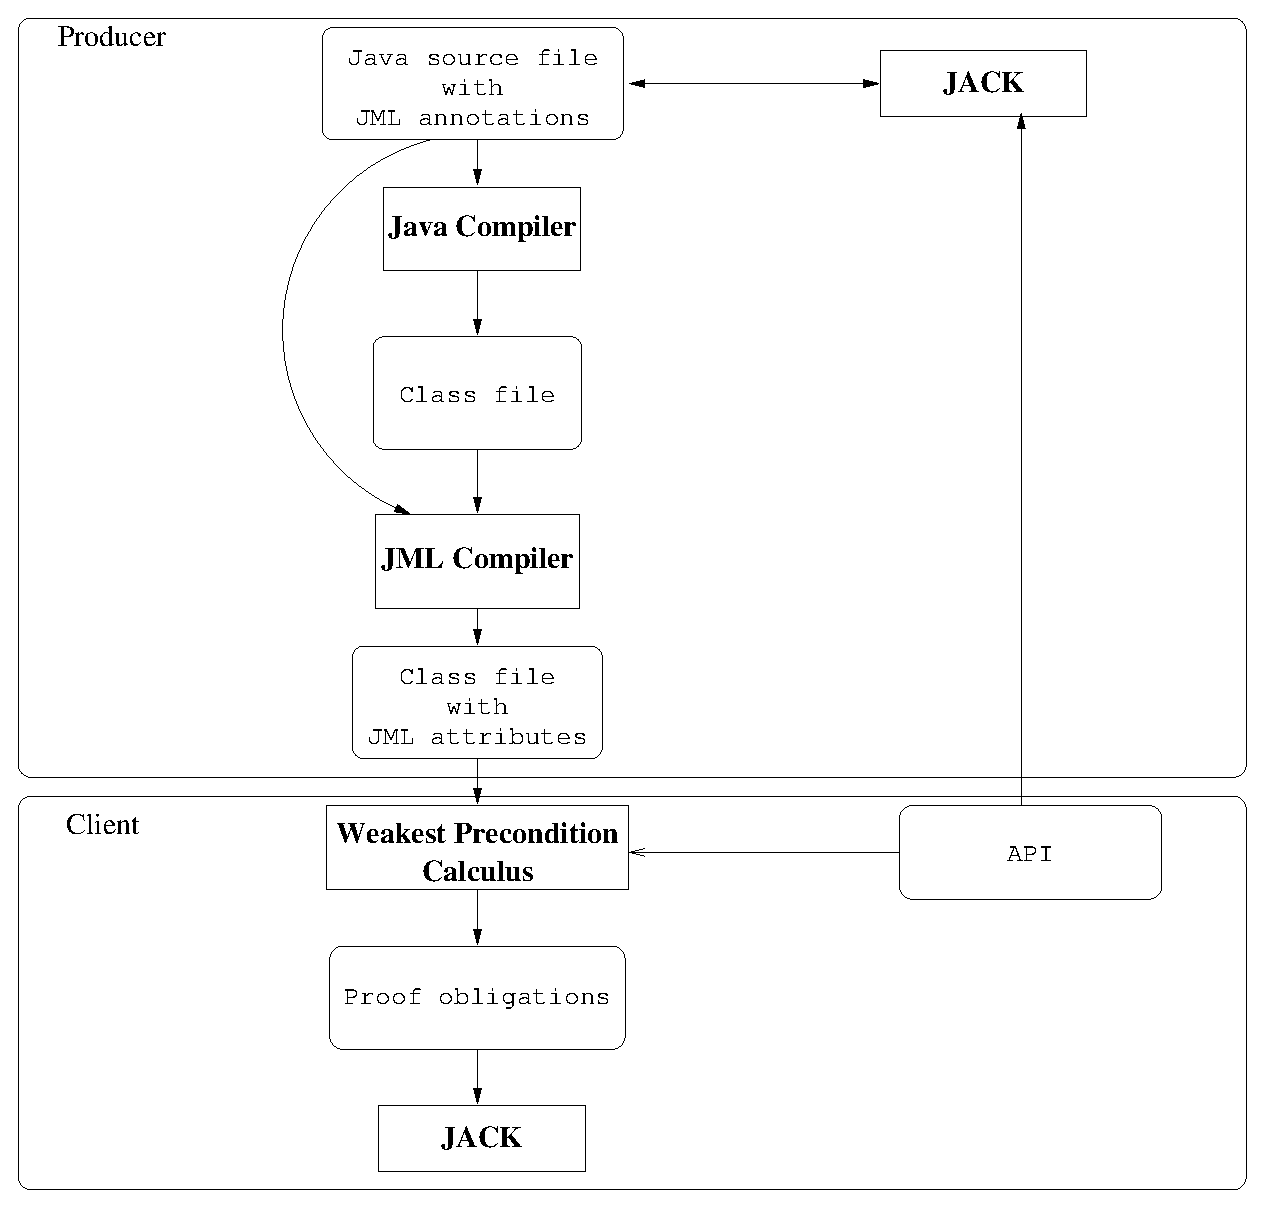
\epsfig{file=architecture.eps, width=\linewidth}
\caption{The overall architecture for annotating and verifying code}
\label{architecture}
\end{center}
\end{figure}
%\clearpage

It describes a process that allows a client to trust a code produced by an untrusted code producer. This approach is especially suitable
 in cases where the client policy involves non trivial functional or safety requirements and thus, an automatic specification inference cannot be applied.

In the first stage of the process the client provides the functional and (or) security requirements to the producer.
 The requirements can be in different form:
\begin{itemize}
\item A specified interface that describes the application to be developed. In that case,
 the client specifies in JML the features that have to be implemented by the code producer.
\item An API with restricted access to some method. In this case, the client can protect its system by restricting the API usage.
For example, suppose that the client API provides transaction management facilities - the API method \texttt{open} for opening and method \texttt{close} for closing transactions. In this case, a requirement can be for no nested transactions.
In this case, the methods \texttt{open} and \texttt{close} can be annotated to ensure that the method \texttt{close} 
 should not be called if there is no transaction running and the method \texttt{open} should not be called if there is already a running transaction. In this scenario we can apply results of previous work \cite{PBBHL}.  
\end{itemize}

%OLD:
% In the development process, the producer uses Jack to check the client requirements and usually has to add JML annotations for this %In both cases, the code producer develops its application and proves that it fulfills the given requirements using Jack; %in most cases, to complete this task, some annotations have to be added to the code 
%e.g. loop invariants, class invariants, method preconditions and postconditions etc. In a standard, application only after specifying enough the source code, 
%have we got the annotated Java source files to feed to the JML compiler.

In the development process, the producer verifies if the client requirements are respected by generating verification conditions
over the source code and usually, he has to add JML annotations for this e.g. loop invariants, class invariants, method preconditions
 and postconditions etc. It is usually only after specifying enough the source code that the annotated Java source and class files are fed to the JML compiler.
% Usually, only after ``specifying enough'' the source code, 
%have we got the annotated Java source files to feed to the JML compiler.

If the annotations are sufficient to prove the code, 
the Java file is normally compiled with a Java compiler to obtain a 
class file. This class file is then extended with user defined attributes that contain the BCSL specification, 
resulting from the compilation of the JML specification in the Java source file. 
At this stage, the Java class files contain all the information that will allow the client to check if the bytecode does not violate 
his requirements. 
 %OLD
%In particular, the client will generate proof obligations from the untrusted annotated bytecode and his security requirements 
%(expressed in a suitable form) as shown in figure~\ref{architecture}. Proof obligations are formulas which, if provable, guarantee the bytecode correctness.
%The latter are then proved , for instance, with JACK (see section \ref{prelim}). If the client succeeds in proving 
%the verification conditions, he can trust the unknown code. Currently the framework does not support sending both the proof and the 
%bytecode to the client, which is the next step in our work.
In particular, the client will generate proof obligations from the untrusted annotated bytecode and his security requirements 
(expressed in a suitable form) as shown in figure~\ref{architecture}. Proof obligations are formulas which, if provable, guarantee the bytecode correctness.
The latter are then proved with a theorem prover (possibly interactively). If the client succeeds in proving 
the verification conditions, he can trust the unknown code. 

Currently the framework does not support sending both the proof and the 
bytecode to the client this being the next step in our work. 

%Actually, our early experiments show that the proof obligations on source and bytecode level are syntactically modulo names and types.   

%OLD
%To implement this architecture, we have defined a compiler from JML to BCSL; the JML compilation results in an extension of the class file format; 
%we have implemented a tool to insert those special attributes in the class file and we have extended the JACK framework to generate proof obligations at bytecode 
%level and to prove them with the plugged JACK provers (as explained in the introduction). 
%The coming sections introduce those features.  

To implement this architecture we use JACK as a verification condition generator both on the consumer and the
producer side. JACK is a plugin for the eclipse\footnote{http://www.eclipse.org} integrated development environment for Java. Originally, the tool was designed as verification condition generator for Java source programs against their JML specification. JACK can interface with several theorem provers (AtelierB, Simplify, Coq, PVS). We have extended the tool with a compiler from JML to BCSL and a bytecode verification condition generator. In the following we introduce the BCSL language, the JML compiler and the bytecode weakest precondition calculus which underlines the bytecode verification condition generator.
 
%the JML compilation results in an extension of the class file format; we have implemented a tool to insert those special attributes in the class file and we have extended 
%the JACK framework to generate proof obligations at bytecode level and to prove them with the plugged JACK provers (as explained in the introduction). 
%The coming sections introduce those features.  


\section{JACK's User Interface}\label{SecUI}

One of the features that distinguish JACK from other program
verification tools is the integration in the IDE Eclipse. This ensures
a seamless integration of formal methods in the application
development process: the application developer does not have to learn
the peculiarities of a new tool, and does not have to switch tools to
apply formal verification techniques.

The integration in Eclipse consists of two parts: an extension of the
standard Java perspective with special JACK-related actions (checking a
specification, calling an automatic prover \emph{etc.}), and a
special JACK perspective to inspect the generated proof
obligations.

\subsection{Extension of the Java Perspective in Eclipse}

The standard Java perspective of Eclipse is extended with several
JACK-specific features. Menus are added to set the defaults for the
different specification constructs. Further, there are buttons and
menu-options to ``compile'' a JML specification, (\emph{i.e.}, type
check and generate proof obligations), call an automatic prover on all
the generated proof obligations (either Simplify or a special
Coq tactic), or change to the special JACK perspective.  

Checking the JML specification is not done in a background mode, while
editing the file (as is done for the type checking of Java);
instead the user has to launch this action explicitly. 
At the time this interface was developed,
adding such automatic checks required too many changes to the
internals of Eclipse, which were not default available. However, in
the mean time such a feature has been developed within the JMLEclipse
project\footnote{See
\texttt{http://jmleclipse.projects.cis.ksu.edu/}.}. This project also
provides syntax highlighting of JML specifications in Eclipse's Java
perspective. All this could be integrated with the JACK interface. 

%It is future work to integrate this with the JACK interface.
%%(\emph{e.g.}\ the JMLEclipse project does not accept the keywords that
%JACK adds to JML. 

Finally, another important constraint is the interface's
responsiveness. An IDE is supposed to be used interactively, and the
developer should never have to wait long for a result. Proof
obligation generation is no problem for this, but calling an automatic
prover on the generated proof obligations can take a significant
amount of time. Therefore, the prover is called in a non-blocking way,
launching a special window that allows to see the progress of the
task.

\subsection{A Proof Obligation Inspection Perspective}

An important feature of JACK is that one can inspect the different
generated proof obligations. Moreover, one does not have to understand
the specific specification language of the prover that is being used;
instead the proof obligations can be viewed in a Java/JML-like syntax
(but of course, one can also choose to see the proof obligations as
they are generated for a specific theorem prover).

\begin{figure}[t!]
%julien: at my desk it makes things bugs....
% \epsfig{file=screen1.ps,angle=270,width=\textwidth}
% the following work better (for me, with the makefile)
\epsfig{file=screen1bis, width=\textwidth}
\caption{JACK's proof obligation inspection perspective}\label{FigJackPerspective}
\end{figure}

%\begin{figure}[th!]
%    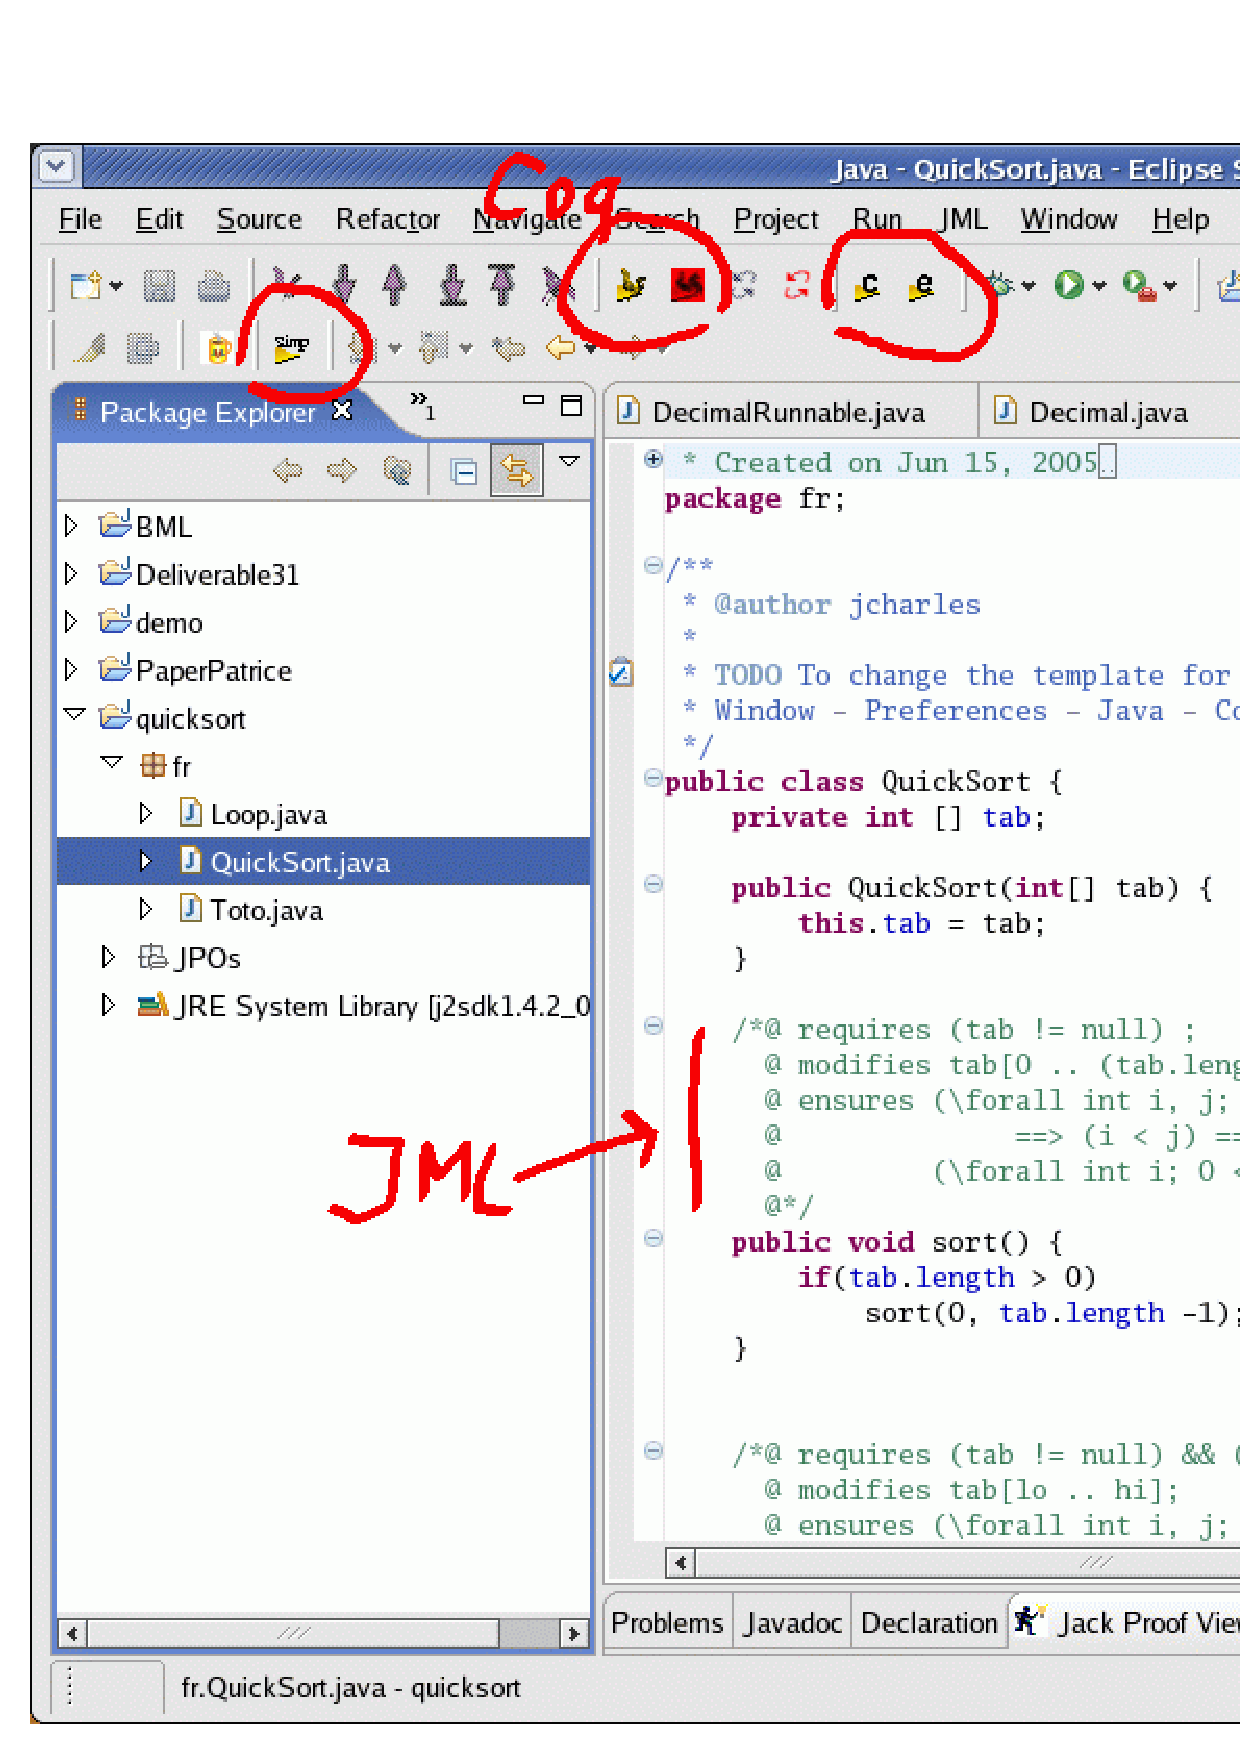
\includegraphics[width=\textwidth]{screen1}
%\caption{JACK's proof obligation inspection perspective}\label{FigJackPerspective}
%\end{figure}
%JACK's proof obligation inspection perspective provides the following information:
%\begin{itemize}
%\item information concerning the current proof status;
%\item the class methods with their lemmas;
%\item the source code; and
%\item the currently selected proof obligation (goal and hypotheses).
%\end{itemize}

Figure~\ref{FigJackPerspective} shows the inspection of a proof
obligation for the method \texttt{sort} in the \texttt{QuickSort}
example of Figure~\ref{FigJMLSpec}. The left upper windows allows one
to browse the proof obligations for the current class. Proven
obligations are ticked, the others are marked with a cross. The right
window shows the original source code, where the path through the code
that corresponds to the current proof obligation is coloured, together
with the relevant part of the method specification. Different colours
are used to indicate different cases, \emph{i.e.}, to distinguish
normal from exceptional execution, and to mark that extra information,
such as a method specification, or the result of a conditional
expression, is available. For example, in
Figure~\ref{FigJackPerspective} one sees the specification of the
private \texttt{sort} method in a pop-up box, used in the public
\texttt{sort} method.

The bottom window shows the proof obligation: the left half contains
the hypotheses, marked with letters indicating their origin,
\emph{e.g.}, a hypothesis marked R originates from the method's
requires clause, while a hypothesis marked L is derived from local
declarations within the method. The right half of the window shows the
actual goal that has to be proven. The window name highlights once
again that this proof obligation originates from the
postcondition. Finally, notice that the proof obligation is displayed
in Java syntax, but buttons are available to change to Coq, Simplify
or PVS syntax.

%\marginpar{MH: Say something about 'manual check' option for proof
%obligations}

The user can use the proof obligation inspection view to inspect the
different (unproven) proof obligations, and to launch different
(interactive or specialised) provers to prove the remaining proof
obligations.


\section{Generating JML Annotations}\label{SecAnnotGen}

While JML is easily accessible to Java developers, actually writing
the specifications of a smart card application is labour-intensive and
error-prone, as it is easy to forget some annotations. There
exist tools which assist in writing these annotations,
\emph{e.g.}~Daikon~\cite{ErnstCGN01} and Houdini~\cite{FlanaganL01}
use heuristic methods to produce annotations for simple safety and
functional invariants.  However, these tools cannot be guided by the
user---they do not require any user input---and in particular cannot
be used to synthesise annotations from realistic security policies.

Within JACK, we have implemented several algorithms to generate
annotations. We can distinguish two sorts of applications for
annotation generation. The first goal is to generate as much
``obvious'' annotations as possible, to reduce the burden of
annotation writing. Given an existing, unannotated, application, one
first tries to generate preconditions automatically, before specifying
the more interesting parts of the specification. The second goal is to
encode high-level properties by encoding these with simple JML
annotations, that are inserted at all appropriate points in the
application, so that they can be checked statically.

JACK implements algorithms for both goals, and both will be described
in this section.


\subsection{Generation of Preconditions and Frame Conditions}
JACK implements two different algorithms to generate ``obvious''
annotations. The first algorithm is a simple static analysis on the
program text, which generates modifies clauses. Whenever it sees
assignments or method calls that change (specification) publicly
visible fields, these fields are added to the method's modifies
clause. The algorithm uses a safe over-approximation: whenever it
encounters references that might be aliased, it will simply generate a
clause \texttt{modifies \bsl everything;}.

JACK also implements an algorithm to generate the minial preconditions
to avoid nullpointer and array-out-of-bounds exceptions. This
algorithm re-uses the implementation of the weakest precondition
calculus: it computes the weakest precondition for the specification
\texttt{exsures (NullPointerException) false} (\texttt{exsures
(ArrayIndexOutOfBoundsException) false}) and inserts this as an
annotation in the code. 

As an example, Figure~\ref{FigAnnotSpec} shows the annotations that
are generated for a fragment of the class QuickSort that was presented in
Figure~\ref{FigJMLSpec}. 
\begin{figure}[t!]
{\small
\begin{verbatim}
public class QuickSort {
  private int [] tab;

  /*@ requires this.tab!=null;
      modifies \everything;
      exsures (Exception ) false;
    @*/
  public void sort() {if(tab.length > 0) sort(0, tab.length -1);}

   /*@ requires this.tab!=null&& 
                0<=j&& j<this.tab.length&&
                0<=i&& i<this.tab.length;
       modifies \everything;
       exsures (Exception ) false;
    @*/
  public void swap(int i, int j) {int tmp; tmp = tab[i]; 
                                  tab[i] = tab[j]; tab[j] = tmp;}

  ...
}
\end{verbatim}
}
\caption{Annotations Generated for a Fragment of Class
\texttt{QuickSort}}\label{FigAnnotSpec} 
\end{figure}
It is important to realise that, even though the specifications that
are generated are not very spectacular, the fact that they can be
generated automatically can help significantly to reduce the burden of
annotation writing.

Notice that the annotation generation can be further improved by doing
some simple analysis on the generated annotations. Often it is the
case that the preconditions that are generated for the fields of the
class are the same for (almost) all the methods. In that case, this
condition is most likely a class invariant, and instead of generating
it as a precondition for each method, it would be more appropriate to
generate a single class invariant. In the class \texttt{QuickSort} in
Figure~\ref{FigAnnotSpec}, this would lead to a clause
\texttt{invariant this.tab!=null;}. It is future work to implement
this improvement.

\subsection{Encoding of Security Policies}

Another problem when writing annotations is that a conceptually simple
high-level property can give rise to many different annotations,
scattered through the code, that encode this property. This is
typically the case for many security policies. Current software
practice for the development of applications for trusted personal
devices is that security policies give rise to a set of rules that
should be obeyed by the implementation. Obedience to these rules is
established by manual code inspection.

However, many of these rules can be formalised as simple automata,
which are amenable to formal verification. Therefore, we propose a
method that given a rule to guarantee a security policy, automatically
annotates an application, in such a way that if the application
respects the annotations then it also respects the security
policy. The generation of annotations proceeds in two phases:
synthesising and weaving.
\begin{enumerate}
\item Based on the security policy we \emph{synthesise} core annotations, 
specifying the behaviour of the methods directly involved.
\item Next we propagate these annotations to all methods directly or
indirectly invoking the methods that form the core of the security
policy, thus \emph{weaving} the security policy throughout the
application. 
\end{enumerate} 




Both the cyclic and acyclic graphs of the bytecode of method \texttt{isMember} at Fig.~\ref{isMemBC} is at Fig. ~\ref{blockBC}. Blocks are represented by boxes. Black arrows stand for relation $\execRel^A$. Dashed arrows stand for the acyclic relation $\execRel$.





\begin{figure}[p]
\begin{center}
\begin{tabular}{rl}
 0 & iconst\_0 \\
 1 & istore\_2 \\
 2 & iconst\_0 \\
 3 & istore\_2 \\
 4 & goto 14 \\
 5 & aload\_0 \\
 6 & getfield \#19 <test/ListArray.list> \\
 7 & iload\_2 \\
 8 & aaload \\
 9 & aload\_1 \\
10 & if\_acmpne 13 \\
11 & iconst\_1 \\
12 & ireturn \\
13 & iinc 2 by 1 \\
14 & iload\_2 \\
15 & aload\_0 \\
16 & getfield \#19 <test/ListArray.list> \\
17 & arraylength \\
18 & if\_icmplt 5  \\
19 & iconst\_0 \\
20 & ireturn \\
\end{tabular}
\end{center}
\caption{the bytecode of method \texttt{isMember}}
\label{isMemBC}
\end{figure}




\section{Support for Interactive Verification}\label{SecInteractive}
When automatic provers fail to solve a proof obligation,
the user can try to change the specifications of the program or
 solve the proof obligation interactively.
Using the interactive verification support of JACK,
the user will be able to solve the proof obligation in case
the automatic prover was not powerful enough or he will be able to analyse 
thoroughly the proof obligation to find the source of the error.
This verification is done mainly with the Coq proof assistant. 

First we will discuss the architecture of JACK's Coq plugin, then its 
integration within the IDE Eclipse. Finally we will talk of
 JACK's specific annotation keyword for interactive verification, the 
\native keyword. 

\subsection{The Coq Plugin}
Proof readability and proof reusability is crucial in interactive 
verification: in automatic verification it is not the case because proof
obligations are simply given to the automatic prover and no concern is made
out of whether the proof obligation is readable or not.
Therefore we developed a set of facilities to
pretty print, to reuse the proofs, especially when the specifications 
have changed to be able to try to replay the proofs, and to the build the proofs.

JACK, uses short variable names in proof obligations as much as possible, 
but in case of ambiguity long variable names are used.
The scope of these disambiguations can be mistaken: JACK generates all 
the names for all the proof obligations of one file in a row whereas 
in interactive verification the variables are only 
used within a single proof obligation.
The Coq Plugin corrects this in redoing the disambiguation for each proof obligation.
This adds better proof readability as the variable names are shorter.
The main pretty printing is done directly through Coq's own pretty printing features. 


A special attention has also been given when generating the proof obligations 
into a file. First it has a human-readable name so the user can retrieve 
the proof obligation with Jack whenever he wants it. 
This way, if the lemma is regenerated or reopened
 the proof it was containing can be replayed 
(and eventually fail if the conditions have changed too much), and it does not have
to be rewritten.
The normal hypothesis are separated from the invariants and
are given different names.
It is specifically useful when a goal has been modified (and considered 
unproved) by the modification of a class invariant. If the proof was not involving
the use of any invariant; it can be replayed without any changing. This facilitates
greatly the reuse of proofs.

One of the key point in interactive verification is the level of difficulty
to manipulate the proof assistant in order to solve a proof obligation.
In order to help the user to build proof scripts that are both intuitive
to read and to make, we have used the tactic mechanism of Coq~\cite{DEL-00-LTAC}.
As JACK generates proof obligations for automatic verification, numerous hypothesis are 
added to help the automatic theorem prover. For interactive verification 
these hypothesis are usually useless. Therefore there are some tactics made
to clean up the proof obligations. There are also tactics to solve proof patterns
generated by JACK: the ones to solve arithmetic goals,
when the solving of a proof leads to an absurd case, the ones to help solving
array specific proof obligations and the ones to solve assignment proof obligations.
This library of tactics\footnote{
A full description of the different tactics is available here:
\texttt{http://www-sop.inria.fr/everest/soft/Jack/doc/plugin/coq/Prelude/} .}
is useful but usually the user likes to define his own application
specific tactics. The Coq Plugin also allows automatic resolution of proof obligations
using generic proof scripts.
A user can define his own tactic in the Coq Plugin in a file 
dedicated to that purpose; so he can use them in the interactive solving or with the 
automatic resolution.








\subsection{JACK with Coq in Eclipse}
An important feature of JACK is that everything can be done inside the same IDE, Eclipse.
The Coq Plugin complies to this rules and to do so it contains an editor for Coq, 
CoqEditor. This permits to solve efficiently the proof obligations generated by JACK as
well as to easily develop user extensions for the Coq Plugin all inside of Eclipse.

Coq editor is a way to interact directly with Coq through Eclipse's Java 
environment. The user can evaluate and edit Coq files within the
Eclipse IDE. It is similar what has been done for Isabelle in 
Proof General Eclipse \cite{WintersteinAL05}, in a more light-weight fashion.
It has keyboard shortcuts similar to CoqIde (the current Coq graphical
interface which is written in OCaml)\footnote{It is available with the
distribution of Coq (\texttt{http://coq.inria.fr}).}. 
CoqEditor has an outline view,
which sums up the structures of the currently edited Coq file 
in a tree-like fashion (especially useful with to see modules hierarchy). 
CoqEditor has also an incremental indexing feature which allows the user
to jump from a keyword to its definition.
Of course, there is syntax highlighting for Coq files 
and one can interactively evaluate a Coq file
as in the usual interactive provers IDE.


\subsection{Towards native specifications}
\begin{figure}[t!]
{\small In JML we define:
\begin{verbatim}
/*@ public native class IntList {
     public native IntList cons (int i);
     public native static IntList create();
     ...
     public native static IntList toList (int [] tab);
   } @*/ \end{verbatim}}

{\small And in Coq:
\begin{verbatim}
Definition IntList := list t_int.
Definition IntList_create : IntList := nil .  
Definition IntList_cons:  t_int -> list t_int ->list t_int := 
            fun (i: t_int) (this: list t_int)  => (i :: this).
... \end{verbatim}}
\caption{The definition of native type \texttt{IntList}}\label{CoqAnnot} 
\end{figure}
Sometimes users would like more expressivity: instead of having
tactics and extensions based solely on Jack's Java logic, a user may want to
build his own logic and use it with JML annotations. That is 
exactly the purpose of the \native construct \cite{Charles06}.

The \native construct is made to express some notions contained within
the annotation directly in the logic of the prover. It can be used 
as \native types and as  \native methods.
A \native method is a specification method that is like a {\tt pure} method 
but  it does not throw any exception and is used uniquely through the specifications. 
A \native type is a type to use with specification methods (\native methods as well as 
JML's {\tt model} methods). Both are references to a constructs 
defined in the proof obligation's target language: usually \native types are bounded to 
types and \native methods to functions definitions.


If we define a \native type IntList and we bind it to a list of integer type 
 (Figure \ref{CoqAnnot}), we can use the list library of the target prover (here Coq) 
in the proofs. The specifications of the
{\tt sort} method can be defined as specifications using our new type 
(Figure \ref{sortnat}). We get more readable annotations;
the annotations are more natural for the user because instead
 of relying upon Java logic over the array, we get it defined directly into
our target proof obligations language syntax.
The user can also define more easily lemmas to help prove some of the proof
obligations and to add automations for proof scripts.


\begin{figure}[t!]
{\small In JML we define:
\begin{verbatim}
//@ ghost IntList list;
/*@ requires (tab!=null) && list.equals(IntList.toList(tab))
    assignable tab[0 .. (tab.length -1)], list;
    ensures list.equals(IntList.toList(tab)) &&
             list.isSorted() && list.isPermutation();
 @*/
public void sort() {if(tab.length > 0) sort(0, tab.length -1);}\end{verbatim}}
\caption{\texttt{Sort} with natives}\label{sortnat} 
\end{figure}






\section{Achievements}
% done. summary
We have  presented an infrastructure for verification of Java bytecode programs   which allows to reason about potentially
sophisticated  functional and security properties and
which benefits from verification over Java source programs. We have also 
introduced the bytecode specification language BML tailored to Java bytecode, a compiler
from the Java source specification language JML to BML and a verification 
condition generator for Java bytecode programs. 
We have shown that the verification procedure is correct w.r.t. a big step  operational semantics of Java bytecode programs. 
Moreover, we have
proven that the verification procedure for Java like programs
and Java like bytecode are syntactically equivalent (modulo names and types). 
%This scheme is actually part of the PCC architecture of the
%European project Mobius\footnote{the site name} which aims to resolve the problems
%of mobile and ubicuous computing via PCC. 
We have developed a prototype of a verification condition generator based on the weakest precondition calculus presented in this thesis, as well 
as a compiler from the corresponding subset of JML to BML.
These two components have been integrated in the JACK \cite{BRL-JACK} verification framework 
developed and supported by our research team Everest at INRIA Sophia Antipolis which has been initially designed for
 the verification of Java source programs annotated with JML specification.

We would like to give a brief description of the implementation of the verification condition generator.
 The extension of the tool to bytecode programs which we added also interfaces these theorem provers. The bytecode 
verification condition generator works as follows. For the verification of a class file containing BML specification, it will generate verification conditions for every
 method of this class including the constructors. For generating the verification conditions concerning a method implementation, first the control flow
 graph corresponding to the bytecode instruction is built. The latter is transformed into an acyclic control flow graph where the backedges are 
removed.
 Then the verification procedure proceeds by generating over every execution path in the control flow graph its corresponding verification conditions. 
For every path which terminates by throwing an uncaught exception, the postcondition is the specified exceptional postcondition for this case. For the paths which terminate normally, 
the normal postcondition is taken. For every path which terminates with an instruction which is dominated by a loop entry and whose direct successor is the same loop entry, the postcondition 
is the corresponding loop invariant. The bytecode verification in Jack uses the intermediate language for the verification conditions and thus, bytecode verification conditions 
 can be translated to several different theorem provers - Simplify \cite{Simpl05DNS} which is an automatic decision procedure, 
the Atelier B and the Coq interactive theorem prover assistants. 

The bytecode verification condition generator benefits also from the original user friendly interface of the JACK tool.  In particular, 
the user can see the verification conditions in his favorite language - Java, Simplify, Coq or B. The lemmas are classified 
to what part of the annotation they refer to, as for instance, a lemma which refers to the establishment of the postcondition, or the preservation of the loop invariant.
The hypothesis in the lemma also hold the index of the instruction from which they originate. 
We have used the prototype of the bytecode verification condition generator for the case studies presented in Chapter \ref{applications:optimComp}.

% JACK (short for Java Applet Correctness Kit) is designed as a plugin for the Java interface development
% environment eclipse. 
%% It was originally tailored to the verification of Java source programs 
%w.r.t. their JML specifications. The tool has an intermediate proof obligation language which allows to extend it easily to interface more 
% theorem provers. Thus, the tool interfaces several theorem provers - Simplify \cite{Simpl05DNS} which is an automatic decision procedure, 
%%the Atelier B and the Coq interactive
%theorem prover assistant. 

\section{Future work}
In the following, we identify the directions for extending the work presented in this thesis

\subsection{Language coverage of the verification condition generator}
The bytecode verification condition generator works only for the sequential fragment of Java. But realistic applications 
rely often on multi - threading which is difficult to verify against a functional specifications or security policies.
One of the important aspects of the correctness of multi - threaded programs is the absence of deadlocks, 
and race conditions. Such properties can be ensured  by type systems \cite{FA99TSL,flanagan00typebased} or static verification based on program logic \cite{FLL02ESC}.  
The absence of deadlock and race conditions is a first step in the verification of the functional correctness of multi threaded programs. In order to build a full 
verification scheme for checking functional correctness more has to be done.
The earliest work for  verification of  parallel programs is  the Owicki and Gries approach   
\cite{nipkow99owickigries}  and the rely - guarantee approach. However, 
the first approach is not modular and requires a large amount of verification conditions while for the second, the annotation procedure can not be automatised.

% Such techniques for reasoning over the correctness of parallel programs  exist.
% One of the first logic - based verification techniques for parallel programs is due to Owicki and Gries 
%\cite{nipkow99owickigries}  in which every point of parallel interference is annotated and then the verification consists in establishing that
% all the possible inter leavings of all the threads respect the annotation. This technique is on one hand not modular as the verification process 
%needs the implementation of every program component and on other hand the number of verification conditions may be very big.
% Another approach is the rely guarantee technique which uses a Hoare style verification conditions \cite{nieto03relyguarantee}.
%There, the program points of interference are annotated not only with the predicate that must hold
%at the point but also with rely and guarantee  conditions which express what conditions the program guarantees to the other threads and what 
%the program requires from the other threads. This technique although tempting because of its modularity and the smaller number of verification conditions is difficult to apply
%as for guessing the rely and guarantee conditions requires an in - depth understanding of the program to be verified.  
Extending our verification scheme for bytecode will certainly be based on a more recent work  where one of the basic concerns is to establish method atomicity  \cite{TES03CF}. 
The notion of a statement atomicity states  that however a statement is interleaved with other parallel programs, the result of its execution will not change.
The atomicity can be  detected via static checking \cite{TES03CF} using type systems. Thus, the program verification process is separated in two parts
- first checking for program atomicity  \cite{TES03CF} are done  
and then verifying the functional correctness using  methodologies for sequential programs as Hoare style reasoning. 
In this last approach in the case of Java, the basic concern is to establish the atomicity of method bodies, i.e. method 
execution does not depend on the possible interleaving with threads.
Recently, E.Rodriguez and al. in \cite{RodriguezDFHLR05} proposed an extension for JML for multi threaded
 programs. Their proposal introduces  new specification keywords which allow to express that a variable is locked or
 that a method is atomic.% Giving the semantics of these keywords is still an ongoing work but we consider that the meaning of these specification constructs does not differ on source and bytecode. 
    
 



\subsection{Property coverage for the specification language}
Another direction which may be pursued as a future work of the thesis  is the extension of the expressiveness of the specification language BML. 
So far, BML supports method contracts - method pre and post  conditions, frame conditions, intermediate annotations as for instance
loop invariants, class specifications as well as special specification operators.
These are very useful aspects which allow for dealing with complex properties and 
gives a semantics on bytecode level  to a relatively small subset of the 
high specification language JML which corresponds to JML Level 0 \footnote{ http://www.cs.iastate.edu/~leavens/JML/jmlrefman/jmlrefman\_2.html\#SEC19}. 
 But it is certainly of interest to support more features of JML in BML
as this will turn the latter language richer. However, the meaning  of JML constructs 
(at least from our experience up to  now) is the same as the meaning of their corresponding part in BML.  

 An important example is the  JML construct for pure methods which has been  identified as  a challenge in the position paper \cite{LeavensLeinoMueller06}. 
 These methods does not modify the program state and thus, pure methods can be used in specifications 
 (only side effect free  expressions may occur in expressions).
 This gives more expressive  specifications as with them, for instance, specification can talk about the result of method invocation or use pure methods
 as a predicate relating their  initial and final state. 
 Formalizing and establishing the meaning of pure methods is difficult and a literature exists for this problem \cite{DarvasMueller06}.
 As we said above, the treatment of pure methods is the same on source and bytecode.

Also, support for specification constructions for alias control is certainly useful  especially because it allows for a modular verification 
of class invariants and frame conditions.
The alias control is guaranteed through ownership type systems which check that only an owner of a reference can modify its contents.
 This can considerably improve the current implementation for the verification of object invariants  \cite{DietlMueller05}.
In particular, our way of proving object invariants is non modular - at every method call the invariants of all visible \todo{say what does it mean visibility}
objects must be valid and they are assumed to hold when the call is terminated; similarly, when a method body is verified in its precondition the invariants of all visible
objects are assumed to hold and at the end of the method body all these invariants must be established. 
In practice, it is very difficult to verify that all the invariants for the all visible objects in a method  hold.
In order to keep the number of the verification conditions reasonable, we check the invariants only for the current object this and the 
objects received as parameters which is not sound.

 
\subsection{Preservation of verification conditions}

So far, we have shown that non-optimizing Java compilation
 preserves the  form of the verification conditions on source and
 bytecode.  We identify two basic directions for future work:
\begin{description}
 \item[Source and non optimized bytecode verification conditions equivalent modulo] % implement the compiler from Java source pogs to bytecode pogs
We have experimented with the verification conditions on source and
 bytecode in JACK and saw that in practice they are almost equivalent
 syntactically. From one part, there are the difference in the types 
 supported on bytecode and source level. For instance, the JVM does not
 provide support for boolean type values which are basically encoded as
 integer values. The same is true for byte and short values.  Another
 difference is the identifiers for variables and fields. For instance, in Java
 names for fields, method local variables and parameters are their identifiers which are given by the
 program developer. On bytecode method local variables and parameters are encoded as elements of the
 method register table and field names are encoded as numbers of the constant
 pool table of the class. A  simple but useful extension to the prototype for
 bytecode verification is a compiler from source proof obligations to bytecode proof obligations
 which overcomes those differences. This can be considered also as a step
 towards the  building a PCC architecture where the certificate generation benefits from
 the source level verification and thus allows for treating sophisticated
 security policies.

\item[Relation between verification conditions on Java source and optimized Java bytecode]
 The equivalence  between verification conditions on source and the corresponding non optimized bytecode is important as it
 allows that bytecode programs  benefit from source verification. In particular, it makes feasible Proof Carrying Code
 for sophisticated client requirements.
 However, a step further in this direction is to investigate the 
 relation between source programs and their bytecode counterpart produced by an optimizing compiler.
 This is interesting for the following reasons.
 It is a fact that interpretation of bytecode on the JVM is slower than execution by its corresponding assembly code. 
 In order to speed up the execution time for a Java bytecode program, one might use 
 a just-in-time compilation which  translates on the fly the bytecode into the machine specific language. However, JIT compilation can potentially slow
 the execution exactly because it does compilation on the fly.  Another possibility is to perform 
 optimizations on the bytecode. Currently, most of the  Java compilers do not support much optimizations.
 However, there do already exist Java optimizing compilers, for instance the Soot optimization framework\footnote{http://www.sable.mcgill.ca/soot/} 
 and most probably the number of the Java optimizing compilers will increase with the evolution of the Java language.
 A first step in the latter direction is the work of C. Kunz et al.\cite{BGKRsas06} who give an algorithm for translating 
 certificates and annotations over a non optimized program into a certificate  and annotation for its optimized version.
 Their work addresses  optimizations like constant propagation, loop induction, dead register elimination etc. 
\end{description}
\subsection{Towards a PCC architecture}

The bytecode verification condition generator and the BML compiler is the first step towards a PCC framework. 
The missing  part is  the certificate format which comes along with the bytecode and which  is the evidence for 
that the bytecode respects the client requirements. Defining an encoding of the certificate should take into account several factors:
\begin{itemize} 
  \item certificate size must be reasonably small. This is important, for instance,  if the certified program comes over a network with a limitted bandwith
  \item certificates must be easily checked. This means that the certificate checker is  small and simple.
	       Of course, the code consumer might not want to spend all of its computation 
	      resources for checking that the certificate guarantees the program conformence to its policies.     
\end{itemize}

Note that the certificate size and its checking complexity are dual: the bigger the certificate is more manageable is the checking process and viceversa. 
The problem becomes even more difficult if the certificate must be checked on the device because of the computational and space constraints.
 


% towards.PCC
% For building a PCC framework from the components cited above 
% % there is still missing the proof certificate, the decision procedure
% that will be used by the producer for the certificate generation and the type checker used by the code
% client for checking the certificate. Important problems in this direction are
% \begin{itemize}
%  \item light weight verification condition generators. In particular, we refer 
%        to verification condition generation techniques which are simple and do not need
%	much computational resources. Because a verification condition generator always
%	form part of the trusted computing base on the client side, building such verification 
%	condition generators is important for on - device checking which rely on limitted computational 
%	resources  
  
%   \item generation of certificates. This is important for several reasons.
%         The certificate may certainly  arrive via the network and should not corrupt the performance 
%  
% 
% %  \item efficient type checker on the client site. This is in particular important 
%         if the device is with limitted resources where a complex certificate checking procedure
%         may corrupt the performance of the device
%        
%     
% \end{itemize}


 %To do this,  it is still missing the proof
%certificate, the decision procedure used by the code producer 
%for building the certificate  as well as the type checker used by the code
%client for checking the certificate. 

% to do. type systems
Another perspective in this direction is how   to encode type systems into the bytecode logic. 
Type systems provide a high level of automation. 
Their encoding in the logic can be useful as the certificate can be generated
 automatically and thus, avoids the user interaction. However, type systems are  conservative in the sense 
that they tend to reject a large amount of correct programs. A possible solution to this problem are hybrid certificates which combine both type systems and program 
logic. In this approach, the unknown code comes supplied with a  derivation in the logic generated potentially with the help of user interaction 
for the parts of the  code which can not be inferred by the type system.   The client side then applies a type inference procedure over  the
 unknown code and once it gets to the place in the parts of the code where the 
type inference does not work but for which there is a derivation in the certificate, he will type check that derivation.   
This is actually an approach which will be adopted in the Mobius project. 


The objective of this thesis was to 
give the basis for the a bytecode verification framework and to show that it is feasible. A further objective, pursued in the European project
 Mobius (short for Ubiquity, Mobility and Security) 
is to build basis for guaranteeing security and trust in program application in the presence of mobile and ubicuous computing. We hope that we have convinced
the reader for the importance of such techniques and in particular of the evolution from source verification to
 low level verification  and the necessity of an interactive verification process for building evidence for the security of unknown applications. 


\bibliographystyle{plain}
\bibliography{bibli,fmco,../specification,/user/mhuisman/home/Research/Everest/Biblio/everest,/user/mhuisman/home/Research/Everest/Biblio/crossrefs}

\end{document}

